% Each picture is one long division. The quotient is aligned by powers of x.
\documentclass[tikz,multi=tikzpicture,border=5pt]{standalone}
\usepackage{lmodern}
\definecolor{placeholder}{HTML}{707880}
\tikzset{every picture/.style={x=1cm,y=.52cm,font=\normalsize},every node/.style={anchor=base,inner sep=0pt},rule/.style={line width=.42pt},zero/.style={text=placeholder}}
\begin{document}
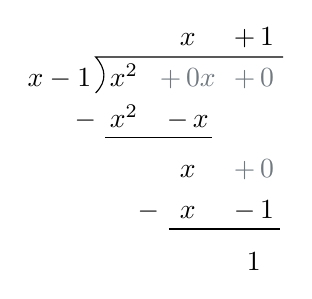
\begin{tikzpicture}
\node at (-.82,0) {$x-1$};
\node at (0,0) {$x^2$}; \node[zero] at (.81,0) {$+\,0x$}; \node[zero] at (1.65,0) {$+\,0$};
\node at (.81,1) {$x$}; \node at (1.65,1) {$+\,1$};
\draw[rule] (-.36,-.16) .. controls (-.21,.13) and (-.23,.44) .. (-.36,.72) -- (2.02,.72);
\node at (-.49,-1) {$-$}; \node at (0,-1) {$x^2$}; \node at (.81,-1) {$-\,x$};
\draw[rule] (-.24,-1.25)--(1.12,-1.25);
\node at (.81,-2.23) {$x$}; \node[zero] at (1.65,-2.23) {$+\,0$};
\node at (.31,-3.23) {$-$}; \node at (.81,-3.23) {$x$}; \node at (1.65,-3.23) {$-\,1$};
\draw[rule] (.57,-3.48)--(1.98,-3.48);
\node at (1.65,-4.5) {$1$};
\end{tikzpicture}
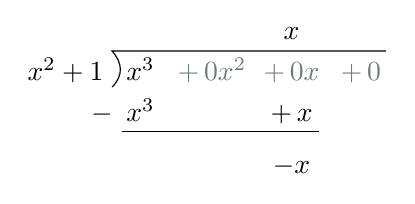
\begin{tikzpicture}
\node at (-.95,0) {$x^2+1$};
\node at (0,0) {$x^3$}; \node[zero] at (.91,0) {$+\,0x^2$}; \node[zero] at (1.92,0) {$+\,0x$}; \node[zero] at (2.8,0) {$+\,0$};
\node at (1.92,1) {$x$};
\draw[rule] (-.36,-.16) .. controls (-.21,.13) and (-.23,.44) .. (-.36,.72) -- (3.12,.72);
\node at (-.49,-1) {$-$}; \node at (0,-1) {$x^3$}; \node at (1.92,-1) {$+\,x$};
\draw[rule] (-.24,-1.25)--(2.27,-1.25);
\node at (1.92,-2.27) {$-x$};
\end{tikzpicture}
\end{document}
